% Document settings and packages
\documentclass[a4paper,12pt]{report}
	\usepackage[utf8]{inputenc}
	\usepackage{graphicx}
	\usepackage{hyperref}
	\usepackage{url}
	\usepackage[acronym]{glossaries}
	\graphicspath{{figures/}}
	
% Acronyms page
\makeglossaries
\newacronym{vpn}{VPN}{Virtual Private Network}
\newacronym{ip}{IP}{Internet Protocol}
\newacronym{ipv4}{IPv4}{Internet Protocol version 4}
\newacronym{ipv6}{IPv6}{Internet Protocol version 6}
\newacronym{tcp}{TCP}{Transmission Control Protocol}
\newacronym{udp}{UDP}{User Datagram Protocol}
\newacronym{gre}{GRE}{Generic Routing Encapsulation}
\newacronym{tls}{TLS}{Transport Layer Security}
\newacronym{ipsec}{IPsec}{Internet Protocol Security}
\newacronym{ssh}{SSH}{Secure Shell}
\newacronym{l2tp}{L2TP}{Layer 2 Tunneling Protocol}
\newacronym{osi}{OSI}{Open Systems Interconnection}
\newacronym{dtls}{DTLS}{Datagram Transport Layer Security}
\newacronym{mipv6}{MIPv6}{Mobile IPv6}
\newacronym{ietf}{IETF}{Internet Engineering Task Force}
\newacronym{sa}{SA}{Security Association}
\newacronym{esp}{ESP}{Encapsulating Security Payload}
\newacronym{ah}{AH}{Authentication Header}
\newacronym{spd}{SPD}{Security Policy Database}
\newacronym{sad}{SAD}{Security Association Database}
\newacronym{pad}{PAD}{Peer Authorization Database}
\newacronym{spi}{SPI}{Security Parameter Index}


\begin{document}
	\title{Virtual Private Networks}
	\author{Bogdan Ionescu}
	\date{\today}
	\maketitle
	\tableofcontents
	
	% Print acronyms page
	\glsaddall
	\printglossary[type=\acronymtype,nonumberlist,style=long]
	
	\chapter{Virtual Private Networks}
	\section{Importance of VPNs}
		In this day and age, networking is everywhere, especially considering the exceedingly fast expansion of the Internet. The Internet, the ultimate network of networks, has radically changed our day-to-day life. Just several years ago, simple everyday habits, such as quickly searching for a piece of information on Google, online shopping, streaming your favorite songs or paying your bills with just a few clicks would have seemed possible only in a distant future. And yet here we are today, achieving even more impressive tasks, making use of all kinds of networks available within our laptops, phones, tablets and even home electronics, thanks to the IoT.
		
		Unfortunately, the Internet's rapid development also comes with a few important drawbacks which are regrettably often overlooked --- the most significant one being cybersecurity. \textit{Cybersecurity} is the protection of computer systems and networks from the theft and damage of hardware, software or electronic data, as well as from the disruption of the services they provide. Most often, networks, full of information, are the first frontier when trying to exploit systems,  which is why network security represents such an important key aspect against cybercrime.
		
		Inevitably, when having any communication over the Internet, a significant amount of data is being sent between you (more precisely, your device) and the other party, commonly a server or another person's device. Although this data can sometimes be quite harmless, such as a quick Google search for a cake recipe or just streaming some music, in some cases it may contain more sensitive and valuable information than you can think of. Personal messages while chatting with a close friend, credit card information when making an online payment, passwords used when logging in to different websites, the video feed recorded by your webcam when having an online conference --- these are only just a few examples of what kind of infomation leaves your private home network when accessing the Internet. Since the Internet is a public network, such data can be easily intercepted by other parties before reaching its destination, which often leads to catastrophic consequences.
		
		By now you might think that if you are using an application which encrypts its data, you should be safe on the Internet. Unfortunately, this is often not the case, as there are many places where things can go wrong. For example, in many messaging systems, messages pass through intermediary parties, such as the application's servers, which store them, from where they are retrieved by the recipient. In such scenarios, data is generally encrypted only in transit --- from the sender to the server, and from the server to the destination. Even if the servers encrypt the data at rest (which, surprisingly, does not always happen), they still must have access to the cryptographic keys used in this process, therefore information is still being vulnerable in case the actual servers are being targeted. Moreover, this allows the third party, or any other organization which has a backdoor to these servers, to freely recognize our data. Such invasion of privacy is prevented by using end-to-end encryption, a system where only the communicating users can read the messages, denying any other third party to access the cryptographic keys needed to decrypt the information.
		
		Even if such encryption is used, with strong cryptographic ciphers, unlikely to be broken in attacks, we still might experience some troubles. Application data that leaves our home network, in order to be routed over networks, will have an \acrfull{ip} header added to it, which contains our public IP address and the destination IP address. These are unique, ISP-issued addresses which can be used to monitor and censor traffic, since every service we try to access will be identified by its IP address. This could also lead to IP address-based geo-blocking and IP range ban, methods often employed by media companies, governments, intelligence agencies and many others.
		
		So far we have only talked about the consequences from the point of view of a casual user, but damages rise significantly in the case of cyber attacks against major businesses, usually leading to huge amounts of loss in revenue. In fact, Juniper Research estimated that the average cost of a data breach in 2020 will exceed \$150 million, as more business infrastructure gets connected \cite{junipercybercrime}. In order to mitigate cyber attacks, they usually maintain one or more private networks inside their offices and only from within these controlled networks employees can access necessary resources. Such resources can actually be part of the same network, thus making transfer of data safe, since everything happens inside the private network, but inevitably some resources, such as cloud services, will be accessed through the Internet. Some employees must also be able to connect to the private network through the Internet even if they are part of another network, in order to access its resources, possibly in case of time-critical emergencies or just to work remotely from their homes. Therefore, many companies need a technology that allows secure communication between their private network and another host across a public network, or even to another different private network, such as communication between two private networks owned by different offices of the same company, located in distant regions.
		
		The solution to all the aforementioned problems, and to many other vulnerabilities while using a public network, is a \acrfull{vpn}.
		
		\section{What Is a Virtual Private Network?}
		Security over networks is usually described by three components: confidentiality, integrity and authenticity. Confidentiality, often achieved by encryption, guarantees that data can only be understood by authorized entities. Integrity ensures that the data has not been modified between these endpoints. Finally, authenticity proves that data originated from an authorized party, and not from another source. Apart from these three, another concept which is often massively desired over public networks refers to anonimity, which assures that information we send out does not divulge our identity. All of these can be achieved by VPNs, if implemented correctly.
		
		A \acrfull{vpn} extends a private network by allowing hosts which are not part of it to send and receive data over a public network, usually the Internet, as if they are directly connected to the private network. VPNs are build by establishing a virtual link of communication between two nodes, one being part of the private network. The second node will forward its traffic to it, the first node acting like a proxy, therefore appearing as the traffic actually originated from within the private network from which it is part of. Since encryption is a common, yet not an inherent part of a VPN connection, this channel of communication is usually called a \textit{tunnel} --- only the two endpoints being able to understand the data passing through it. 
		
		Classified by the type of topology of connections, defined by the location of the two endpoints, VPNs usually are of three types: site-to-site, point-to-point (sometimes also called host-to-host), which are the most common, and a combination of the two, point-to-site.
		
		Site-to-site VPNs, illustrated in figure \ref{fig:site-to-site_VPN}, establish a tunnel between two whole networks, therefore allowing any authorized host in any of the two networks to make use of it. Such architecture is frequently used by businesses to securely connect networks owned by the same company in different regions.
		\begin{figure}[h]
			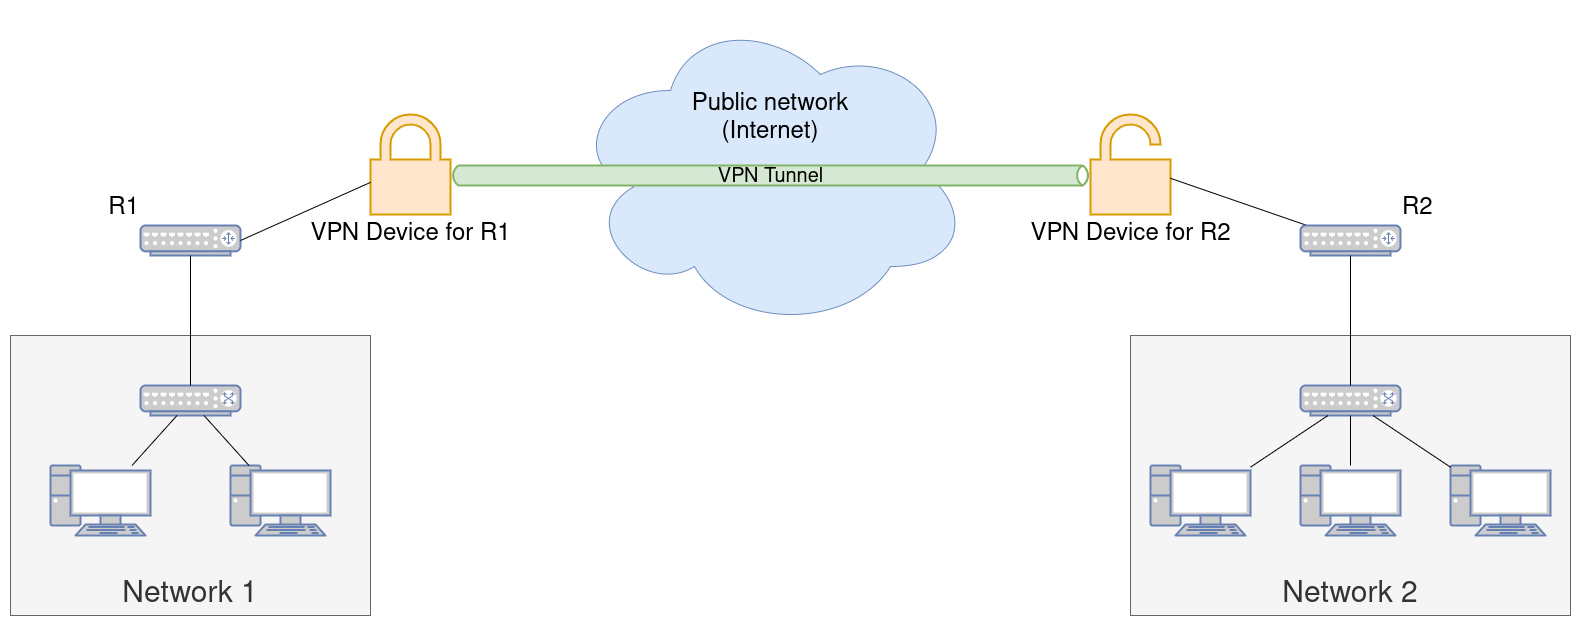
\includegraphics[width=\textwidth]{site-to-site_VPN}
			\centering
			\caption{In this site-to-site architecture, the two VPN devices establish a secure tunnel through the public network. Since traffic must be encrypted from one site to another, the two VPN endpoints, placed in this case after the routers, are responsible for securing data before it crosses the public network. VPN technology can also be directly embedded in routers, removing the need for two additional devices.}
			\label{fig:site-to-site_VPN}
		\end{figure}
		
		Advantages of site-to-site VPNs include scalability, being quite straightforward to add another site, or more devices inside one of the networks, and high availability, as the VPN tunnel does not depend on a device inside the network to initiate and maintain the secure connection. However, for regular users who wish to remain as private as possible, site-to-site VPNs have a quite serious disadvantage. Since traffic is secured just as it leaves the site, by the VPN device or router, data is still vulnerable in the network until it reaches this point, or after it was decrypted, at the other site. As a result, anyone who can intercept our traffic at these stages is a potential threat. Although this scenario is not likely to happen in a business office, it is very probable, for example, for someone who wishes to secure his data from a public place which offers free Internet connection, such as a coffee shop or restaurant.
		
		Point-to-point VPNs (figure \ref{fig:point-to-point_VPN}) establish a secure tunnel between two single hosts in usually separate networks, encryption and decryption taking place only at these points, therefore providing end-to-end encryption and eliminating the aforementioned risk present with site-to-site architectures.
		\begin{figure}[h]
			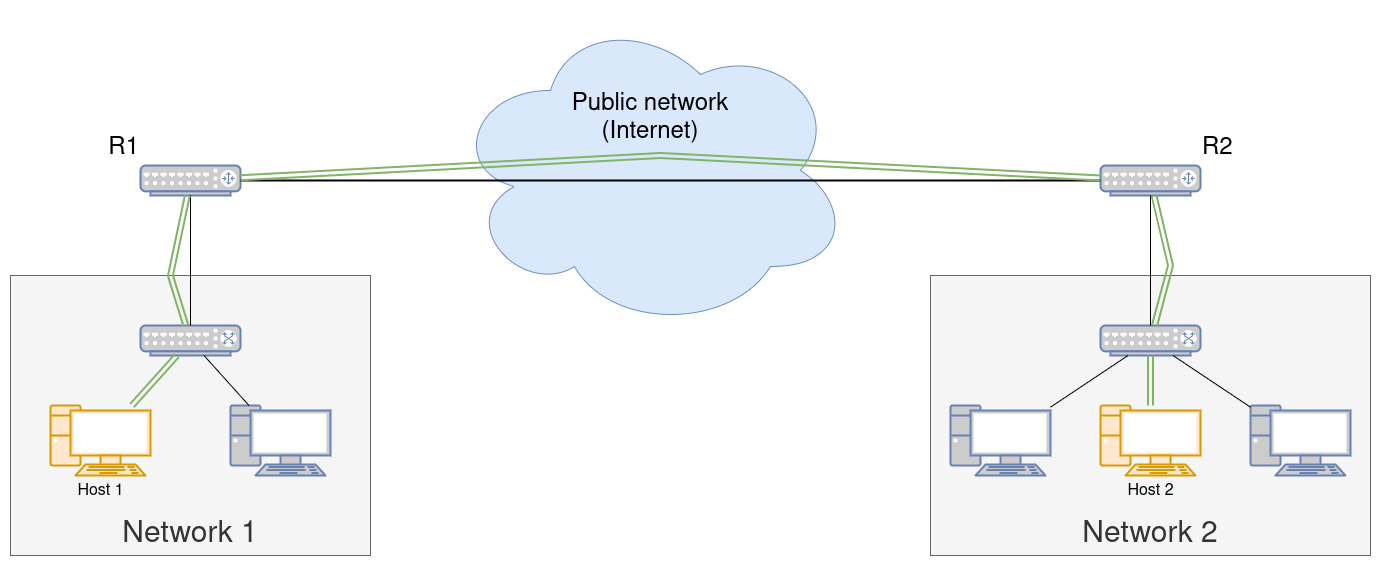
\includegraphics[width=\textwidth]{point-to-point_VPN}
			\centering
			\caption{A point-to-point VPN tunnel between two hosts. The tunnel is usually initiated by one endpoint, but it is dependent on both; if one of the endpoints is down or unreachable, no tunnel can be established.}
			\label{fig:point-to-point_VPN}
		\end{figure}
		
		Point-to-point VPNs are used to form traditional consumer VPNs, where a user establishes a secure tunnel between his device and a server, which is then used as a proxy to access resources, possibly again through the Internet. If this traffic is intercepted, its origin could only be traced back to the proxy server, not the authentic source, which is the other endpoint of the tunnel. This can only be identified by those who have access to the proxy server, in addition to all the decrypted traffic routed through it. Although some VPN service providers claim that they do not log such traffic when clients use their servers, this sometimes is hard to believe. Such risks, along with the fact that VPN providers charge for their services, prompt users to rely on self-hosted VPNs, in which they own the proxy server. In this case, it is the user's job to install and manage the VPN software on both the proxy server and the other endpoint.
		
		\section{Tunneling Protocols}
		The two endpoints of a VPN tunnel do most of the work, being responsible with managing the tunnel and making sure that communication through it is possible. In order for it to actually function, they must modify the regular network packets received from the clients, making sure they are routed to the other endpoint, not to their actual destination, and also provide encryption, if desired. From an original network packet only important information is kept, usually either the network or the transport layer, discarding other layers. This fragment is often called the payload packet, because it is then used as a payload for the final packet. If encryption is used, some portion or the entire payload packet can be modified. This process of encapsulating a packet inside another packet is called \textit{tunneling}, achieved by \textit{tunneling protocols}.
		
		For example, IP in IP \cite{rfc2003} is a tunneling protocol which encapsulates an IP datagram within another IP datagram, as shown in figure \ref{fig:ip-in-ip_packet}. The source IP in the outer IP header will correspond to the entry point of the tunnel, while the destination IP will reveal the exit point, therefore guaranteeing that the packet will be routed to the other VPN endpoint. Except to the encapsulator decrementing the TTL field in the inner IP header, the packet payload remains unchanged during its delivery to the tunnel exit point. Once there, decapsulation takes place, removing the outer IP header and reconstructing the original packet, which will be sent to its original destination.
		\begin{figure}[h]
			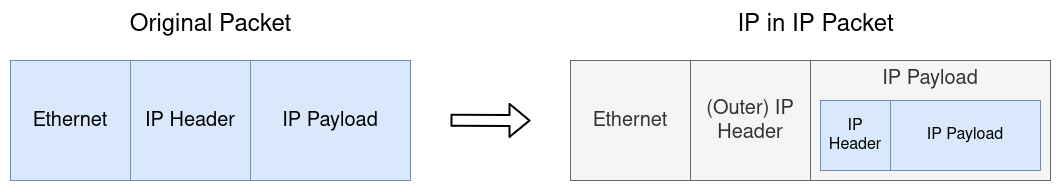
\includegraphics[width=\textwidth]{ip-in-ip_packet}
			\centering
			\caption{IP in IP encapsulates the IP layer (IP header and payload) from the original packet within another IP packet. To differentiate between the two IP headers, the first one is often called the outer IP header.}
			\label{fig:ip-in-ip_packet}
		\end{figure}
		
		\acrfull{gre} \cite{rfc2784}, a protocol fairly similar to IP in IP, developed by Cisco Systems, and Layer 2 Tunneling Protocol (L2TP) \cite{rfc2661} are just another two examples of tunneling protocols frequently used. However, just like IP in IP, all of these protocols do not provide any confidentiality or integrity. They just encapsulate the data received, without modifying it in order to provide encryption. To achieve this, they generally rely on other protocols.
		
		Internet Protocol Security (IPsec) \cite{rfc6071}, Transport Layer Security (TLS) \cite{rfc8446} and Secure Shell (SSH) \cite{rfc4253} are the most often used protocols for secure network services over an insecure network. A key difference between these three protocols is the OSI layer at which they operate. While IPsec is generally considered a network layer protocol, TLS and SSH depend on a reliable stream of bytes and are therefore implemented over TCP, making them layer 5 or above, or just application layer protocols in the TCP/IP suite. The fact that IPsec performs at a lower layer than the rest and it is not dependent on TCP increases its flexibility and capabilities, being able to secure any transport layer protocol, such as UDP. Datagram Transport Layer Security (DTLS) \cite{rfc6347} was also developed to implement TLS over UDP. Tunneling over UDP is sometimes preferred to avoid the TCP meltdown problem (also known as TCP over TCP), in which tunneling a TCP-encapsulating payload induces a dramatic loss in transmission performance (even up to 20\%)\cite{tcpmeltdown}. OpenSSH, an open source suite of secure networking utilities based on SSH avoids the meltdown by decapsulating and re-encapsulating TCP, only sending the payload through the tunnel \cite{opensshmeltdown}.
		
		IPsec, TLS and SSH use a wide variety of strong cryptographic algorithms, providing robust authentication, confidentiality and integrity, amongst many other services. All three of them support tunneling and are currently used to establish and maintain secure tunnels across many networks worldwide. However, the more complex IPsec is still the most viable and preferred option for tunneling, especially for site-to-site VPNs, while TLS and SSH are better for secure remote access, being more straightforward and easier to setup.
		
	\chapter{Internet Protocol Security}
	\section{Components}
		The goal of Internet Protocol Security (IPsec) is to provide security at the network layer, being used worldwide to deploy a variety of VPNs, therefore guaranteeing either secure traffic between networks or in case of remote access, or end-to-end security. It is also often used by other protocols (e.g. L2TP, MIPv6, GRE) to protect some or all of their traffic.
		
		IPsec is not a single protocol, but rather a set of network protocols, each one with critical and specific tasks, working together to achieve the main goal. The complex IPsec protocol suite can be broken into three essential parts which will be thoroughly explained in the next sections:
		\begin{itemize}
			\item \textbf{Security Associations} define the security services and attributes of a connection shared by two network entities
			\item \textbf{Authentication Header} provides connectionless data integrity and data origin authentication for IP datagrams (hereafter referred to as just integrity) \cite{rfc4302}
			\item \textbf{Encapsulating Security Payload} can provide both data confidentiality and integrity, and limited traffic flow confidentiality \cite{rfc2406}
		\end{itemize}
		
		Although a decent part of the IPsec stack is already directly embedded into the Linux kernel, guaranteeing efficient packet processing with minimum overhead, some daemons are still required in user space, generally those regarding Security Associations.
		
	\section{Security Associations}
	IPsec provides data confidentiality and integrity through the two fundamental security protocols previously mentioned, the Authentication Header (AH) and Encapsulating Security Protocol (ESP). Since a VPN device might handle many secure streams of data with different hosts at the same time, when an IP datagram employing AH and/or ESP arrives, how does it know which set of security parameters (cryptographic algorithm, key and policies) to use for that particular connection? Moreover, both AH and ESP support a wide variety of cryptographic systems, and therefore the two endpoints must agree on which algorithm to employ, and perhaps generate and exchange cryptographic keys. As you can see, many attributes and policies must be negotiated and bound to a specific connection between two entities before establishing and using a secure tunnel. This is achieved by Security Associations. 
	
	A Security Association (SA) is a relationship between two or more network entities that describe how the entities will utilize security services to communicate securely. This relationship is represented by a set of information that can be considered a contract between the entities, agreed upon and shared between them \cite{rfc2408}. 
	
	An SA describes only one-way traffic, so, in order to secure typical bi-directional communication between two IPsec-enabled systems, a pair of SAs (one in each direction) is required \cite{rfc4301}. Information is stored in a database, where each SA is uniquely identified by a triple consisting of a Security Parameter Index (SPI), an IP Destination Address, and a security protocol (AH or ESP) identifier. The SPI is a random generated 32-bit value used by a receiver to identify the SA to which the incoming packet should be bound, and is a mandatory field in the ESP and AH headers.
	
	A model defined in RFC 4301 outlines three databases in order to store SA information: the Security Policy Database (SPD), the Security Association Database (SAD), and the Peer Authorization Database (PAD) \cite{rfc4301}.
	
	\subsection{Security Policy Database}

% Print bibliography
\bibliographystyle{abbrv}
\bibliography{bibliography}


\end{document}